\chapter{Discussion}

Chapter~\ref{chpt:ao_tools} details the robust and generalised nature of Microscope-AOtools as well as its accessible implementation within the Microscope-Cockpit UI. The results in Sections~\ref{sec:Aurox_biology} and \ref{sec:DeepSIM_biology} demonstrate significantly improved image quality and resolution, most notably in deep in challenging, live samples as shown in Section~\ref{sec:DeepSIM_biology}. However, no implementation is without limitations and it is worthwhile spending some time discussing them.

\section{Limitations of Microscope-AOtools}
\label{sec:limitations}

\subsection{Zernike mode fitting accuracy}
\label{subsec:zernike_accuracy}

Many the setup methods for Microscope-AOtools outlined in 
Section~\ref{sec:set_up_methods} and the direct wavefront correction 
outlined in Section~\ref{subsec:system_correction} rely on the Zernike 
modes generated from the \textit{AOtools} Python package and the method 
described in Section~\ref{subsec:zernike_mode_measurment} to determine the 
Zernike mode amplitudes present in a phase 
wavefront\cite{townson2019aotools}. It is therefore worth investigating the 
accuracy of this fitting for determining the amplitude of Zernike modes 
present. In theory, measuring the Zernike mode amplitudes present in a 
wavefront image created with known Zernike mode amplitudes using 
\textit{AOtools} should be trivial and yield the same Zernike mode amplitudes 
exactly. Measuring the Zernike mode amplitude present is done using the 
method described in Section~\ref{subsec:zernike_mode_measurment}, but in this 
case the simulated wavefront image created using \textit{AOtools} takes the 
place of the measured phase wavefront, $\Phi(x,y)$. 

The simplest test of the accuracy of the Zernike mode amplitude fitting  
follows thusly. \textit{AOtools} is used to create a wavefront image with 
amplitude 1 radian (i.e. $\alpha_{j} = 1$) of a particular Zernike mode. The 
Zernike mode amplitudes present in the wavefront image is then measured and 
the percentage error between the measured and simulated Zernike mode 
amplitudes is recorded. This process is repeated 50 times for all Zernike 
modes up to radial order, $n = 10$. Figure~\ref{fig:zernike_fitting_accuracy} 
shows the results of this experiment on wavefront images of various sizes. In 
no case is the expected Zernike mode amplitude returned exactly - there is 
always some degree of error in the Zernike mode amplitude measurement. 
Zernike modes with an even azimuthal frequency appear to perform either 
considerably worse or better than Zernike modes with either an odd or zero 
azimuthal frequency. All non-zero azimuthal frequency Zernike modes display a 
trend of increasing percentage error with radial order. The magnitude of 
percentage error also decreases with increasing simulated wavefront size. 

Interestingly, there is often a clear split in percentage error between 
Zernike modes with positive and negative even azimuthal frequencies. This is most visible in 
Figure~\ref{fig:Zernike_fitting_percentage_error_one_mode_256_shape} but it 
can be observed in some radial orders in all the simulated wavefront sizes 
shown in Figure~\ref{fig:zernike_fitting_accuracy}. This observed difference 
in performance between these Zernike modes occurs because positive even 
azimuthal frequencies have a component of variation aligned with 
either the $x$ or $y$ axis whereas negative even azimuthal frequencies do 
not. Zernike modes with a positive even azimuthal frequencies are vulnerable 
to a class of discretisation error where some of the principle variation in 
the simulated wavefront shape falls between pixels and is therefore not 
captured by the discrete representation of the Zernike mode. Odd azimuthal 
frequency Zernike modes do not exhibit this splitting since positive and 
negative odd azimuthal frequencies both have some component of variation 
along the aligned with either the $x$ or $y$ axis. Therefore, odd azimuthal 
Zernike modes always suffer from this class of discretisation error. For 
smaller simulated wavefront sizes, this split in the even azimuthal frequency 
Zernike modes is less visible at higher radial orders because other, less 
geometrically determined, discretisation errors dominate the overall 
percentage error measurements.

\begin{figure}[h]
	\centering
	\begin{subfigure}{0.48\textwidth}
		\centering
		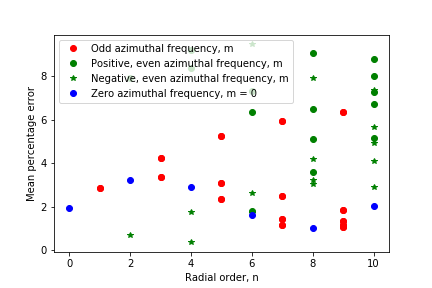
\includegraphics[width=\linewidth]{images/Zernike_fitting_percentage_error_one_mode_32_shape_radial_azimuthal_pos_neg.png}
		\caption{}
		\label{fig:Zernike_fitting_percentage_error_one_mode_32_shape}
	\end{subfigure}
	\begin{subfigure}{0.48\textwidth}
		\centering
		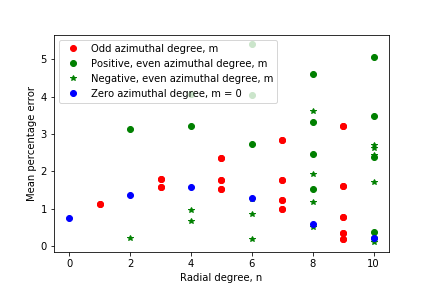
\includegraphics[width=\linewidth]{images/Zernike_fitting_percentage_error_one_mode_64_shape_radial_azimuthal_pos_neg.png}
		\caption{}
		\label{fig:Zernike_fitting_percentage_error_one_mode_64_shape}
	\end{subfigure}
	
	\begin{subfigure}{0.48\textwidth}
		\centering
		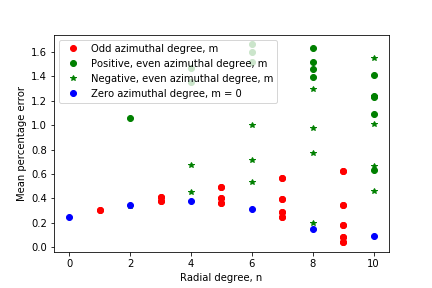
\includegraphics[width=\linewidth]{images/Zernike_fitting_percentage_error_one_mode_128_shape_radial_azimuthal_pos_neg.png}
		\caption{}
		\label{fig:Zernike_fitting_percentage_error_one_mode_128_shape}
	\end{subfigure}
	\begin{subfigure}{0.48\textwidth}
		\centering
		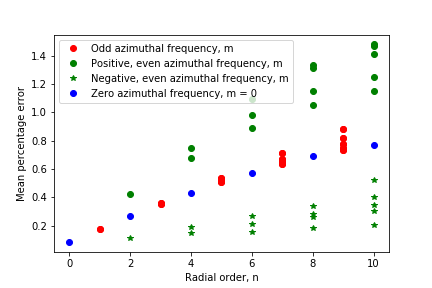
\includegraphics[width=\linewidth]{images/Zernike_fitting_percentage_error_one_mode_256_shape_radial_azimuthal_pos_neg.png}
		\caption{}
		\label{fig:Zernike_fitting_percentage_error_one_mode_256_shape}
	\end{subfigure}
	\caption[The effect of image size on Zernike mode fitting accuracy]{The 
		effect of image size on Zernike mode fitting accuracy. Each 
		subfigure shows the percentage error in the Zernike mode 
		measurement and the linear regression of all Zernike mode 
		measurements for images of size \textbf{(a)} $32\times32$ pixels 
		\textbf{(b)} $64\times64$ pixels \textbf{(c)} $128\times128$ pixels 
		\textbf{(d)} $256\times256$ pixels}
	\label{fig:zernike_fitting_accuracy}
\end{figure}

A wavefront may be dominated by a single Zernike mode, but they are almost 
never composed entirely of one Zernike mode. 
Figure~\ref{fig:Zernike_fitting_percentage_error_random_modes_repeat_resize_factor_1} shows the mean percentage error in the Zernike mode amplitude 
measurement for 50 wavefronts, $256\times256$ pixel size, generated with 
random amplitudes for Zernike modes up to radial order, $n = 10$. Clearly, 
having multiple modes present simultaneously adds a degree of variance to the 
amplitude measurement accuracy as well as an overall increase in the error 
magnitude.

It is a time-consuming process for \textit{AOtools} to generate wavefront 
images of sizes greater than $256\times256$ pixels, typically about a $0.1-1$ 
seconds per image depending on the overall size and number of Zernike modes 
simulated. In order to increase the speed of fitting, acquired wavefront 
images are often resized. This too has an effect on Zernike mode accuracy 
fitting since the resizing function bins multiple pixels together and takes 
their mean, effectively smoothing the wavefront. 
Figures~\ref{fig:Zernike_fitting_percentage_error_random_modes_repeat_resize_factor_2}-\ref{fig:Zernike_fitting_percentage_error_random_modes_repeat_resize_factor_8} show the same set of wavefronts used for the results in 
Figure~\ref{fig:Zernike_fitting_percentage_error_random_modes_repeat_resize_factor_1}, except that the wavefronts were resized by varying factors prior to 
the Zernike modes amplitude measurements. Clearly, the resizing factor is 
inversely proportional to the overall Zernike mode fitting accuracy.

The splitting in fitting error between positive and negative even azimuthal 
frequencies is 
once again observed, and it is observed for all resizing factors. 
A splitting in fitting error is also observed in 
Figure~\ref{fig:zernike_fitting_accuracy_resize} between positive and 
negative odd azimuthal frequencies which was not present previously. One 
might suspect that this is due to the order in which the image axes are 
integrated along using \textit{scipy}'s $trapz$ function. However, the error splitting presented in 
Figure~\ref{fig:zernike_fitting_accuracy_resize} between positive and 
negative azimuthal frequencies is preserved even when the order in which 
the axes are integrated along is reversed. Another reasonable candidate 
for suspicion might be the function used to 
resize the wavefront. If this were the source of this difference in fitting 
errors, it should not occur in 
Figure~\ref{fig:Zernike_fitting_percentage_error_random_modes_repeat_resize_factor_1} since the simulated wavefronts used in this dataset have not been 
resized. This difference in fitting errors may be a result of some internal 
preference within \textit{AOtools}' \textit{phaseFromZernikes()} function 
used to generate the simulated wavefronts. Alternatively, this may reflect a 
genuine preference in the Zernike mode amplitude measurements in complex 
wavefronts for azimuthal frequencies less than 0.

\begin{figure}[h]
	\centering
	\begin{subfigure}{0.48\textwidth}
		\centering
		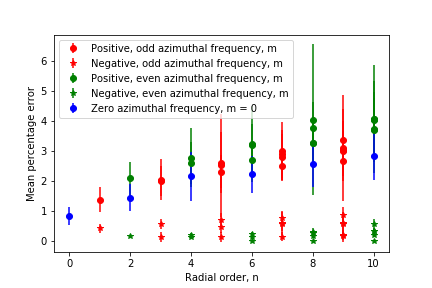
\includegraphics[width=\linewidth]{images/Zernike_fitting_percentage_error_random_modes_repeat_resize_factor_1_order_radial_azimuthal.png}
		\caption{}
		\label{fig:Zernike_fitting_percentage_error_random_modes_repeat_resize_factor_1}
	\end{subfigure}
	\begin{subfigure}{0.48\textwidth}
		\centering
		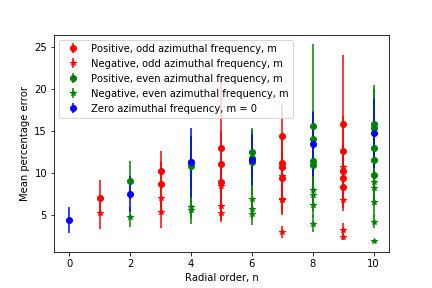
\includegraphics[width=\linewidth]{images/Zernike_fitting_percentage_error_random_modes_repeat_resize_factor_2_order_radial_azimuthal.png}
		\caption{}
		\label{fig:Zernike_fitting_percentage_error_random_modes_repeat_resize_factor_2}
	\end{subfigure}
	
	\begin{subfigure}{0.48\textwidth}
		\centering
		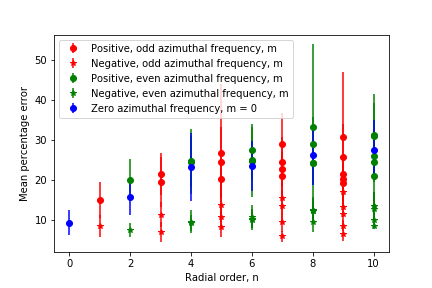
\includegraphics[width=\linewidth]{images/Zernike_fitting_percentage_error_random_modes_repeat_resize_factor_4_order_radial_azimuthal.png}
		\caption{}
		\label{fig:Zernike_fitting_percentage_error_random_modes_repeat_resize_factor_4}
	\end{subfigure}
	\begin{subfigure}{0.48\textwidth}
		\centering
		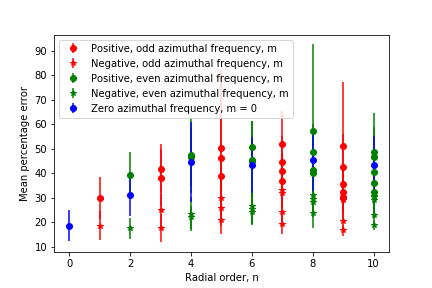
\includegraphics[width=\linewidth]{images/Zernike_fitting_percentage_error_random_modes_repeat_resize_factor_8_order_radial_azimuthal.png}
		\caption{}
		\label{fig:Zernike_fitting_percentage_error_random_modes_repeat_resize_factor_8}
	\end{subfigure}
	\caption[The effect of image resizing on Zernike mode fitting 	
	accuracy]{The effect of image resizing on Zernike mode fitting accuracy. 
		Original images of size $256\times256$ pixels was generated with 
		random amplitudes for Zernike modes up to radial order, 
		$n = 10$. Each subfigure shows the percentage error in the Zernike 
		mode measurement and the linear regression of all Zernike mode 
		measurements for images resized by \textbf{(a)} $1$ i.e. no resizing 
		\textbf{(b)} $\frac{1}{2}$ i.e $128\times128$ pixels \textbf{(c)} 
		$\frac{1}{4}$ i.e $64\times64$ pixels \textbf{(d)} $\frac{1}{8}$ i.e. 
		$32\times32$ pixels} \label{fig:zernike_fitting_accuracy_resize}
\end{figure}

The accuracy of the Zernike mode amplitude fitting is a limiting factor in two key areas. Firstly, the accuracy of the Zernike mode fitting is one of the limiting factors to acquiring an ideal control matrix and, therefore, the ideal characterisation assay shown in Figure~\ref{fig:characterisation_assay_ideal}. Secondly, the accuracy of the Zernike mode fitting is one of the limiting factors to acquiring a perfectly flat wavefront through direct wavefront sensing correction.

\subsection{Sensorless correction accuracy}
\label{subsec:sensorless_accuracy}

In order to make sensorless correction accessible to users the entire 
workflow detailed in Section~\ref{subsec:sensorless_correction} is 
automated. The image quality metric is measured for each image and Python's 
\textit{scipy}'s \textit{curve\textunderscore fit} 
functionality\cite{virtanen2020scipy} is used to fit a Gaussian function of 
the form:

\begin{equation}\label{eq:gaussian}
f(x) = (\Delta - \eta) + \eta e^{-\frac{\left(x-\mu\right)^{2}}{2\sigma^{2}}},
\end{equation}

to the data, where $\Delta$ is the offset value, $\eta$ is the 
normalisation constant, $\mu$ is the mean, and $\sigma$ is the standard 
deviation. The Zernike mode amplitudes applied and the image quality metric 
measurements are used as the $x$ and $f(x)$ variables respectively. 
\textit{scipy}'s \textit{curve\textunderscore fit} functionality then 
estimates the values of $\Delta$, $\eta$, $\mu$, and $\sigma$ which give 
the best fit to the data. An amplitude $\mu$ of the current Zernike mode is 
then applied to obtain the optimum correction for that mode. It is necessary to 
constrain the values which these parameters can take, otherwise it is 
possible for the automation to go awry.

Figure~\ref{fig:zernike_fitting_only_current_power_metric_no_fit_2} shows 
some sample image quality metric values acquired from a correction routine 
on a \textit{Drosophila} neuro-muscular junction preparation similar to 
that shown in Section~\ref{sec:DeepSIM_biology}, acquired on the DeepSIM 
setup. Here the metric measurements were acquired for oblique astigmatism 
(Noll index 5) using the Fourier Power metric from 
Section~\ref{subsec:fourier_power_metric} and the sampled Zernike mode 
amplitudes were $[-2,2]$ radians. If \textit{scipy}'s 
\textit{curve\textunderscore fit} functionality is applied with no 
constraints, the fitting shown in 
Figure~\ref{fig:zernike_fitting_current_power_metric_no_bound_2} is 
obtained. Clearly, there are two problems with this fit. Firstly, the value 
of $\mu$ is $-688$ radians. This is a frankly absurdly high aberration, 
certainly not physically possible for the sample type and depth of imaging in 
question, and not an aberration amplitude the ALPAO-69 DM on DeepSIM (or any 
microscopy deformable mirror) is capable of applying. Secondly, the fit has 
allegedly found a minimum opposed to the desired maximum image quality for 
this mode. 

Imposing the constraint that $\mu \in [z_{l}, z_{u}]$ yields 
Figure~\ref{fig:zernike_fitting_current_power_metric_range_bound_2}. Here 
$z_{l} = z_{min} - 0.25(z_{max}-z_{min})$ and $z_{u} = z_{max} + 
0.25(z_{max}-z_{min})$ where $z_{max}$ and $z_{min}$ are the maximum and 
minimum Zernike mode amplitudes applied. The amplitude acquired is of a 
sensible order of magnitude, $1.85$ radians, however the fit still acquires 
a minimum. Imposing the constraint that $\eta \in [0, \infty)$ 
yields Figure~\ref{fig:zernike_fitting_current_power_metric_bound_2}. These 
constraints guarantee that the value of $\mu$ is both of a sensible 
order of magnitude and corresponds to a maximum. 

It is worth noting that the image quality amplitudes for data points labelled 
``Measured metric values'' in Figure~\ref{fig:sensorless_fitting_accuracy} 
were obtained from images acquired with the corresponding Zernike mode 
amplitudes applied. By contrast, the data points labelled ``Zernike amplitude 
for maximum quality'' are obtained from the theoretical image quality metric 
value according to the obtained fit (i.e. $f(\mu)$) and not from an acquired 
image. They do not represent the image quality obtained when applying the 
corresponding Zernike mode amplitude, only the calculated Zernike amplitude 
for maximum image quality.

\begin{figure}[h]
	\centering
	\begin{subfigure}{0.48\textwidth}
		\centering
		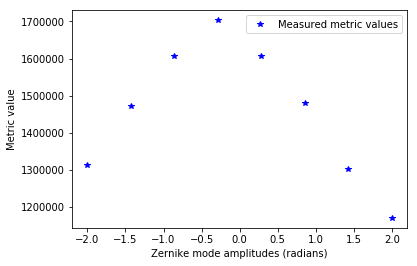
\includegraphics[width=\linewidth]{images/zernike_fitting_only_current_power_metric_no_fit_2.png}
		\caption{}
		\label{fig:zernike_fitting_only_current_power_metric_no_fit_2}
	\end{subfigure}
	\begin{subfigure}{0.48\textwidth}
		\centering
		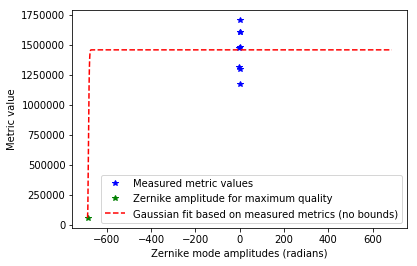
\includegraphics[width=\linewidth]{images/zernike_fitting_current_power_metric_no_bound_2.png}
		\caption{}
		\label{fig:zernike_fitting_current_power_metric_no_bound_2}
	\end{subfigure}
	
	\begin{subfigure}{0.48\textwidth}
		\centering
		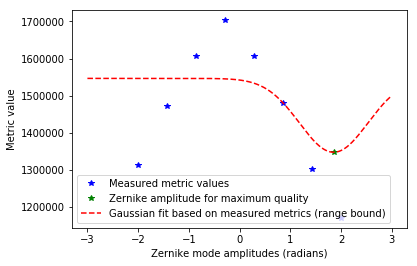
\includegraphics[width=\linewidth]{images/zernike_fitting_current_power_metric_range_bound_2.png}
		\caption{}
		\label{fig:zernike_fitting_current_power_metric_range_bound_2}
	\end{subfigure}
	\begin{subfigure}{0.48\textwidth}
		\centering
		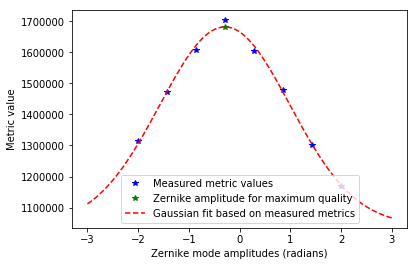
\includegraphics[width=\linewidth]{images/zernike_fitting_current_power_metric_bound_2.png}
		\caption{}
		\label{fig:zernike_fitting_current_power_metric_bound_2}
	\end{subfigure}
	\caption[Effect of parameter bounds on sensorless correction fitting accuracy]{Effect of parameter bounds on sensorless correction fitting accuracy. Metric measurements were acquired for Zernike mode 5 (Noll index) using the Fourier Power metric from Section~\ref{subsec:fourier_power_metric} \textbf{(a)} Measured metric values \textbf{(b)} Gaussian fit with no parameter bounds \textbf{(c)} Gaussian fit with bound on $\mu$ \textbf{(c)} Gaussian fit with bound on $\mu$ and $\eta$}
	\label{fig:sensorless_fitting_accuracy}
\end{figure}

Of course, these constraints do not guarantee a good fit to the data, but 
they do eliminate some sources of fitting error. If the sample aberration is 
primarily from one source - i.e. spherical aberration mismatch - then 
correcting for aberration modes with smaller amplitudes can prove challenging 
since the image quality is already heavily degraded. Similarly, if the fit 
for one mode is poor and leads to an incorrect Zernike mode amplitude being 
applied, this can bias future image quality measurements and prevent 
correction of subsequent Zernike modes. The first case explains why the order 
Zernike modes are corrected in, specified by the user in the interface shown 
in Figure~\ref{fig:DM_sensorless_ao_parameters}, is important. The second 
case explains the existence of the ``Reset DM'' and ``Apply last pattern'' 
buttons in Figure~\ref{fig:DM_methods_cockpit}. ``Reset DM'' returns all 
actuators to their default 0 position. ``Apply last pattern'' applies the last 
recorded actuator pattern applied to the DM. Actuator patterns applied 
through ``Reset DM'' are not recorded. These buttons allow a user to toggle 
between the calculated sensorless correction pattern and no correction 
pattern (i.e. all mirror actuators have no voltage applied). 

For a sensorless correction routine which has failed due to, for example, an 
incorrect correction for one mode has caused a run-away degradation of the 
image quality, this will be visually apparent. Often an incorrect or run-away 
sensorless routine will result in a decrease in image contrast, overall image 
intensity, and the loss of fine structures due a decrease in resolving power. 
For samples with point objects, such as beads or single molecule mRNA, 
characteristic PSF distortions may be visible. 
Figure~\ref{fig:sensorless_unsuccessful_end} shows the results of an 
unsuccessful sensorless correction routine performed on the Alexa488 channel 
of bovine pulmonary artery endothelial cells (F36924, Invitrogen), where 
Alexa488-phalloidin was used to stain F-actin. 
Figure~\ref{fig:sensorless_unsuccessful_end} displays poorer contrast, lower 
intensity, and overall lower resolution compared to 
Figure~\ref{fig:sensorless_unsuccessful_start}.

\begin{figure}[h]
	\centering
	\begin{subfigure}{0.48\textwidth}
		\centering
		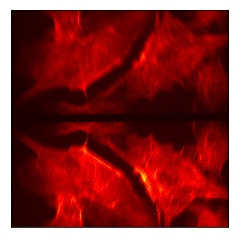
\includegraphics[width=\linewidth]{images/sensorless_unsuccessful_start.jpg}
		\caption{}
		\label{fig:sensorless_unsuccessful_start}
	\end{subfigure}
	\begin{subfigure}{0.48\textwidth}
		\centering
		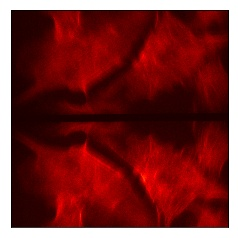
\includegraphics[width=\linewidth]{images/sensorless_unsuccessful_end.jpg}
		\caption{}
		\label{fig:sensorless_unsuccessful_end}
	\end{subfigure}
	
	\begin{subfigure}{0.48\textwidth}
		\centering
		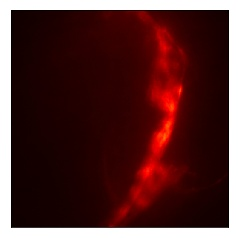
\includegraphics[width=\linewidth]{images/sensorless_successful_start.jpg}
		\caption{}
		\label{fig:sensorless_successful_start}
	\end{subfigure}
	\begin{subfigure}{0.48\textwidth}
		\centering
		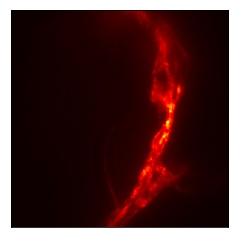
\includegraphics[width=\linewidth]{images/sensorless_successful_end.jpg}
		\caption{}
		\label{fig:sensorless_successful_end}
	\end{subfigure}
	\caption[Visual distinction between unsuccessful and
	successful sensorless correction routines]{Visual
		distinction between successful and unsuccessful sensorless
		correction routines. \textbf{(a)} A bovine pulmonary artery
		endothelial junction before an unsuccessful sensorless
		correction routine \textbf{(b)} A bovine pulmonary artery
		endothelial after an unsuccessful sensorless correction
		routine. \textbf{(a)} and \textbf{(b)} are displayed on the
		same colour scale and show the Alexa488 channel staining
		F-actin. \textbf{(c)} A \textit{Drosophila} neuro-muscular
		junction before a successful sensorless correction routine
		\textbf{(d)} A \textit{Drosophila} neuro-muscular junction
		after a successful sensorless correction
		routine. \textbf{(c)} and \textbf{(d)} are displayed on the
		same colour scale and show the neuron, visualised with Horseradish 
		Peroxidase (HRP) conjugated to Alexa568 fluorophore.}
	\label{fig:sensorless_routine_success_failure}
\end{figure}

In a successful sensorless correction routine, the improvement in image 
quality will be visually apparent. Typically, this manifests as increased 
image contrast, overall image intensity, and additional fine structures becoming 
observable. Where a structured illumination pattern has been applied 
during correction, such with IsoSense, the illumination pattern maybe become 
visible. Figure~\ref{fig:sensorless_successful_end} shows the results of a 
successful sensorless correction routine performed on the Alexa488 channel of 
a \textit{Drosophila} neuro-muscular junction, prepared as described in 
Section~\ref{subsec:DeepSIM_sample_prep}. 
Figure~\ref{fig:sensorless_successful_end} shows enhanced contrast, higher 
overall intensity and additional fine structure compared to 
Figure~\ref{fig:sensorless_successful_start}.
